% This is a sample document using the University of Minnesota, Morris, Computer Science
% Senior Seminar modification of the ACM sig-alternate style. Much of this content is taken
% directly from the ACM sample document illustrating the use of the sig-alternate class. Certain
% parts that we never use have been removed to simplify the example, and a few additional
% components have been added.

% See https://github.com/UMM-CSci/Senior_seminar_templates for more info and to make
% suggestions and corrections.

\documentclass{sig-alternate}
\usepackage{graphicx}
\usepackage{color}
\usepackage[colorinlistoftodos]{todonotes}
\usepackage{float}
\usepackage{wrapfig}

%%%%% Uncomment the following line and comment out the previous one
%%%%% to remove all comments
%%%%% NOTE: comments still occupy a line even if invisible;
%%%%% Don't write them as a separate paragraph
%\newcommand{\mycomment}[1]{}

\begin{document}

% --- Author Metadata here ---
%%% REMEMBER TO CHANGE THE SEMESTER AND YEAR AS NEEDED
\conferenceinfo{UMM CSci Senior Seminar Conference, December 2015}{Morris, MN}

\title{Applications of Memristors}

\numberofauthors{1}

\author{
% The command \alignauthor (no curly braces needed) should
% precede each author name, affiliation/snail-mail address and
% e-mail address. Additionally, tag each line of
% affiliation/address with \affaddr, and tag the
% e-mail address with \email.
\alignauthor
Bailey Denzer\\
	\affaddr{Division of Science and Mathematics}\\
	\affaddr{University of Minnesota, Morris}\\
	\affaddr{Morris, Minnesota, USA 56267}\\
	\email{cssxxxx00000@morris.umn.edu}
}

\maketitle
\begin{abstract}

Recently, advances in traditional computing have begun to decelerate as CMOS based computing is reaching physical barriers to scaling.  This has resulted in less than spectacular improvements to performance, energy efficiency, and density.  Some researchers and companies are starting to see alternative computing architectures as viable alternatives to continue the incremental improvements to computing performance.  One such technology that has recently gained interest is the memristor developed by a Hewlett Packard research team headed by R. Stanley Williams in 2008.  These memristors are being developed in order to implement the crossbar array that has the potential to replace integrated circuits.  

\end{abstract}

\keywords{Memristor, Crossbar Array, computation-in-memory, ITIR, non-volatile, memristive}

\section{Introduction}
\label{sec:introduction}


{Needs more work}
Section two of this paper will first give background information on the memristor which will go over its properties as well as briefly cover its history.  A short introduction to the crossbar array will also be provided in the background.  In section 3 one of the applications of the memristor that makes use of the crossbar array will be covered along with some results of simulations using the architecture compared to conventional computing.  Another application called 1T1R that uses memristors in a more conventional approach without the introduction of the crossbar array will also be described in section 4.  The 1T1R section will also be provided with information on the read and write properties of the memristor.  The paper will then be concluded with section 5.
\section{Background Information}
\label{sec:body}


\subsection{The Memristor}
\label{sec:body}
%\label{sec:typeChangesSpecialChars}
The \textit{memristor} is a \textit{non-volatile} (retains information without power supply) memory that retains a state of resistance depending on the history of applied voltage and current.  It is constructed by placing a layer of highly resistive Titanium Dioxide, $TiO_2$, and a conductive layer of deoxigenized $TiO_{2-x}$, which has positively charged oxygen vacancies, between two electrodes.  These electrodes would most likely be made of platinum and would be part of the crossbar array which will be covered later.  The state of the memristor is altered by passing current through it.  

	A simplified explanation of how this works is as follows.  When a positive voltage is passed through the electrode on the $TiO_{2-x}$ side of the memristor it will cause vacancies to be pushed down into the $TiO_2$.  This results in the $TiO_{2-x}$ increasing in thickness while the $TiO_2$ shortens.  This increase in width of the conductive region and decrease in width of the resistive region significantly reduces the overall resistance as resistance of a material is determined by both its resistive properties and overall length.  The overall width of a memristor is on the order of nm, so it doesn't take much of a change in size of the resistive layer to have a large impact on the resistance.  This results in the memristor having a $R_{On}/R_{Off}$ ratio > 1000, where $R_{Off}$ and $R_{On}$ are the resistances of the memristor that correspond to 0 or 1, respectively.

The memristor was originally hypothesized as the fourth missing circuit element by Chua in 1971, with the others being the resistor, capacitor, and inductor \cite{Chua}.  The theoretical memristor specifies a linkage between magnetic flux and charge.  It was not until recently in 2008 that claims of the physical realization of the memristor were made by R. Stanley Williams's research team at Hewlett Packard \cite{MemFound}.  There has been debate over whether the 2008 memristor really is the theoretical memristor.  The 2008 "memristor" was not the first device created to exhibit memristive properties, however these devices were never claimed to be memristors.  Leon Chua replied to these criticisms in 2011 by stating that all memristive memories can be classified as memristors.   In 2015 Vongher claimed that the current "memristor" is more than likely another implementation of existing memristive memory types, as the conceptual memristor is not possible without magnetic induction \cite{MemNotFound}.  The HP memristor is likely another implementation of oxidation based RRAM, which uses compounds with similar properties to the memristor to store information as resistance.  This should not effect the results of the research though, as it would appear that the physical properties of the "memristor" are true to the explanation given above, and that the criticism is that the "memristor" is not equivalent to the original theoretical memristor.  For simplicity and to avoid confusion I will continue to refer to the HP device as the memristor as that is what the research I'am covering calls it.

\subsection{Crossbar Array}
\label{sec:mathEquations}

When reading research on memristors it is rare to not find mention of the crossbar array.  The crossbar array is simply a collection of switches arranged in a matrix pattern. It was originally invented by HP in 2001.  From then on HP researchers were searching for a switching material with a high enough Off/On ratio to work with it.  Implementing a nano-scale crossbar array was the motivation behind the development of the memristor by R. Stanley Williams's team \cite{MemFound}.  The interest in the crossbar array is due in part to its impressive scaling capabilities (down to ~5 nm) and its simplicity allows it to be cheaply manufactured \cite{Hamdioui:2015:MBC:2755753.2757210}.  More information will be provided on the crossbar array in the CIM section. (Still thinking about where everything should go, might move all crossbar array things up here).

\subsection{Advantages of Memristors}
\begin{figure}
  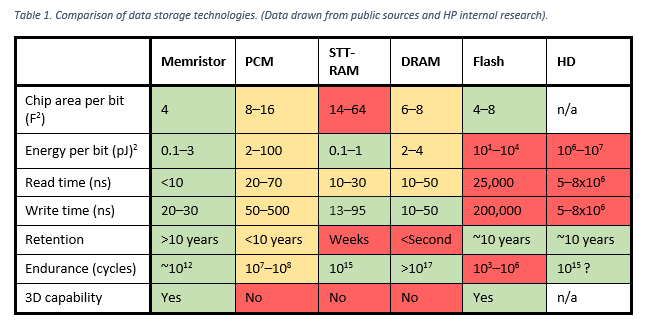
\includegraphics[width=\linewidth]{Comparison-of-Data-Storage-2.png}
  \caption{Comparison-of-Data-Storage-2.}
  \label{fig:DATA}
\end{figure}
\label{sec:inlineEquations}

Figure \ref{fig:DATA} provides a chart of some of the advantages memristors have over other memory storage types \cite{HPmemStuff}.  They have significant advantages in density, read/write time, data retention, cycles (endurance), energy consumption, and the crossbar arrays allow them to be densely stacked into three dimensional crossbar arrays.  Not shown in the chart, memristors have also drawn particular interest as they can potentially be cheaply manufactured using techniques for manufacturing traditional CMOS (Complementary metal-oxide semiconductor).  They effectively combine the advantages of the other storage types into one.

%\section{Memristor Based Architectures}



\section{CIM - Computation in Memory}
\label{sec:citations}

Memristors are not restricted to applications as memory storage.  CIM (computation in memory) is being proposed by \cite{Hamdioui:2015:MBC:2755753.2757210} as a replacement for traditional Von Neumann (VN) architecture for use in data-intensive applications.  Figure \ref{fig:crossbar} gives a simple visual for both VN and CIM architecture.  With traditional architecture processing and data storage are performed in physically separate locations.  This results in the need for large amounts of data transfer between the two.  Von Neumann architecture has some draw backs that CIM architecture can address.  For data intensive computations, having large amounts of data being transferred back and forth between the processor and memory can result in the processors being unable to reach their maximum performance as the processor needs to wait for information transfer, and energy inefficiency as the data transfer can be costly.  It is estimated that communication of data takes up 70 to 90\%\ of energy consumption in VN architecture, with the rest being used for actual computation \cite{Hamdioui:2015:MBC:2755753.2757210}. This is a result of the processor-memory bottleneck, often called the Von Neumann bottleneck.  Within the crossbar array that CIM utilizes, the memristors can be dynamically chosen to be used for either gates or data storage.  This allows large portions of the crossbar array to be set up so that data necessary to a computation can be physically stored next to the memristors that have been converted into gates.  This removes the need to be constantly access things like SRAM which have high energy consumption, poor density, and information bottle-necking.  The motivation behind realizing a CIM architecture is to eliminate the communication bottleneck, support massive parallelism, and reduce energy inefficiency.  

A more succinct overview of the advantages of CIM is as follows:

A) Tightly integrated (scalable to ~5nm) computation-in-memory crossbar
architecture supporting massive parallelism.

B) Little to no leakage.  Current VN architectures suffer from increased leakage with increased scaling as they rely heavily on SRAM caches.

C) Significant performance improvement at lower energy
and area.
\begin{figure}[h!]
  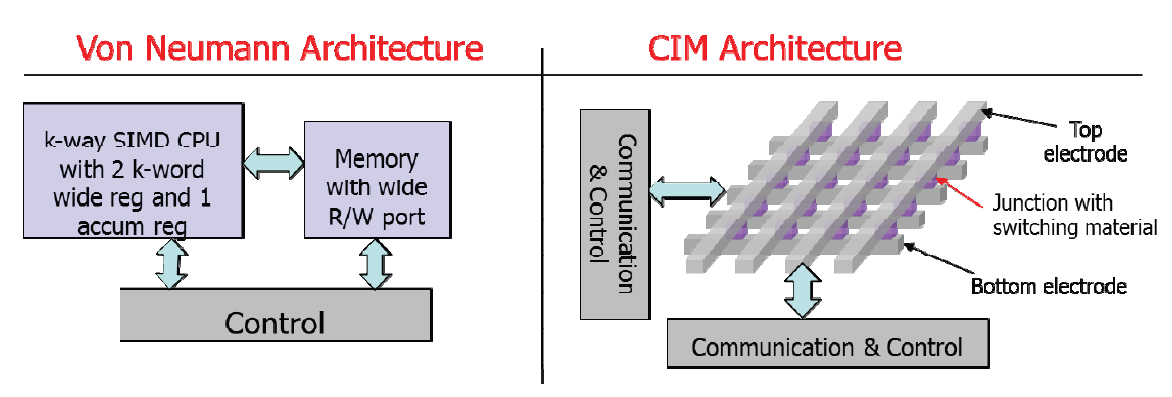
\includegraphics[width=\linewidth]{crossbarexmp.png}
  \caption{Von Neumann architecture on left, CIM on right.}
  \label{fig:crossbar}
\end{figure}


\subsection{Basic Design}
In CIM the computation and data storage are integrated in a crossbar array.  A crossbar array is constructed out of electrodes in a tic-tac-toe pattern with (for example) the horizontal bars being above and the horizontal bars being below.  There is a small gap between them though, allowing memristors to be placed between them at the junctions.

\begin{figure}
  \begin{center}
  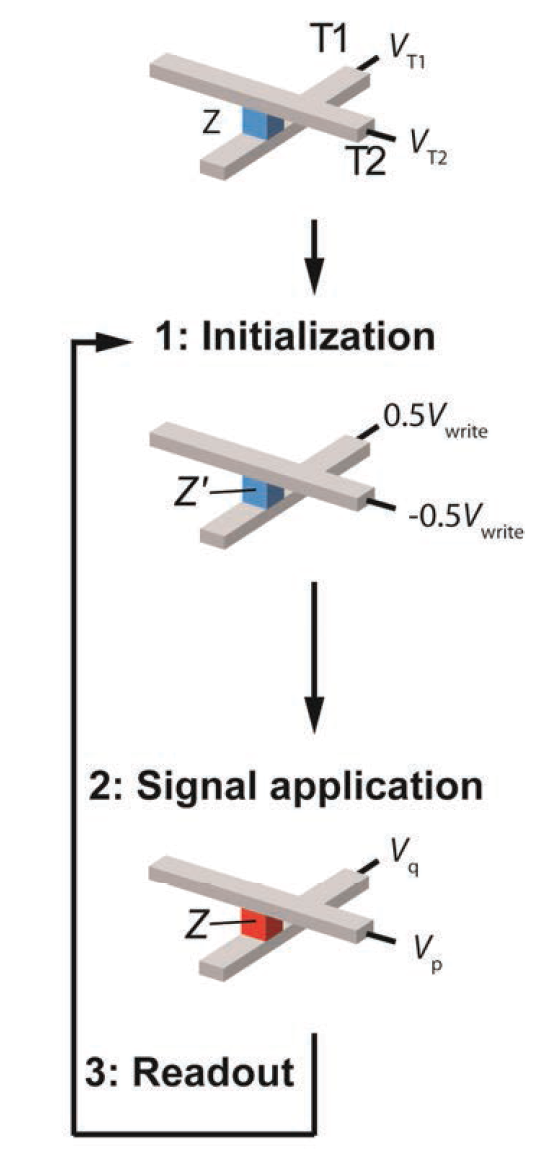
\includegraphics[scale=.2]{inmemcrossbar.png}
  \caption{IMP}
  \end{center}
  \label{fig:inmemcrossbar}
\end{figure}

One of the more promising approaches for performing computations in a crossbar array is (material) implication logic (IMP).  A short explanation of how IMP works is as follows.  Input signals as voltages $ Vp = \pm \frac{1}{2} V_{write} $ and $ Vq = \pm \frac{1}{2} V_{write} $ are applied to the terminals T1 and T2 in Figure \ref{fig:inmemcrossbar} (I'am unsure why this reference is not correct), where $V_{write}$ is a specified voltage to be applied during a write procedure.  This operation will store the resistance state of Z.  In an example where we want to set Z to a value corresponding to bit 1:

1. Init device Z to '1' $(VT1 = + \frac{1}{2} V_{write}, VT2 = -\frac{1}{2} V_{write}$)

2. $Z' = p$ IMP $q (VT1 = Vq, VT2 = Vp)$

3. Read $Z'$

\subsection{Results on Large Data-sets}
\label{sec:theoremLikeConstructs}

\begin{table}[h!]
  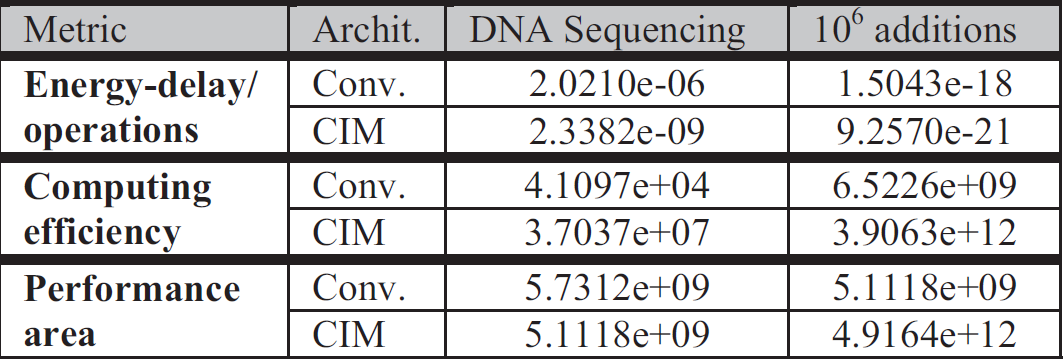
\includegraphics[width=\linewidth]{resulttable.png}
  \caption{Results of simulated data-sets}
  \label{tab:results}
\end{table}

\ref{tab:results} displays the simulated results between conventional and CIM architecture from \cite{Hamdioui:2015:MBC:2755753.2757210}.  The DNA sequencing results were computed by performing a common solution for comparing two DNA sequences in which a sorted index of reference DNA is created in order to identify the locations of matches or mismatches in another sequence.  In the particular case set up by Hamdioui et al. they are comparing 200 GB of DNA data to 3GB of healthy reference. The other example is for $10^6$ parallel addition operations.  The first row of the table represents the the energy-delay product per operations, the second row the computation efficiency defined as the number of operations per required energy, and the third row is the number of operations per area. 

(Frustratingly, the research paper appears to not have units for these rows)
%\subsection{1T1R}
%\label{sec:caveatForExperts}

%Another useful application for memristors is RRAM cells which could potentially replace current forms of memory such as SRAM, DRAM, and Flash memory.  [2] proposes to construct RRAM (resistive random access memory) using a standard CMOS (complementary metal-oxide semiconductor) transistor paired with a memristor.  

%(Still figuring out how to condense down the information from the research paper on this topic)

\begin{figure}
  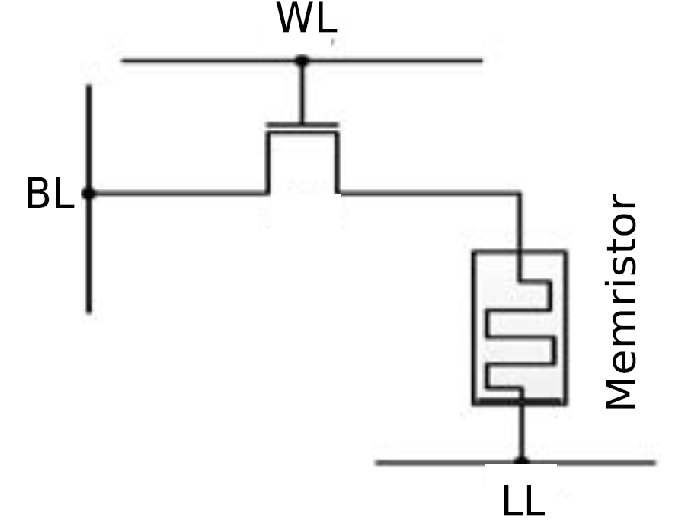
\includegraphics[scale=.29]{1t1real.png}
  \caption{1T1R cell}
  \label{fig:crossSwitch}
\end{figure}

\section{1T1R}
One of the main problems with the crossbar array is the sneak path problem.  Since electricity always looks for a path with the least resistance, there is little preventing the previously described crossbar array from having what is called a sneak path.  This results when an alternative path is made when reading/writing where instead of going through the desired memristor, the current may instead travel through different memristors.  There are multiple ways of dealing with this, but one method in particular is the 1T1R cell as proposed by Zangeneh et al. \cite{Zangeneh:2012:PEM:2206781.2206786}.  It stands for 1 transistor, one resistor (in this case the resistor is a memristor) and has some parallels with DRAM cells, as they are made up of one transistor, one capacitor.  A 1T1R equivalent cell during a write operation is shown in \ref{fig:crossSwitch}.  Like DRAM, the proposed 1T1R architecture has a wordline to select a row of cells and a bitline to select columns.  During a write a voltage $V_{DD}$ is applied to the wordline, and a positive or negative voltage is applied across the memristor for writing 1 or 0 logic.  This is done by either charging the bitline to $V_{DD}$ (for logic 1) or discharging it to 0 $V$ (for logic 0), and applying a voltage $\frac {V_{DD}}{2}$ at node LL.


\subsection{Read/Write Properties of 1T1R}
This subsection will provide the four main equations for the read and write models, regarding the time to read/write and the energy to read/write.  Comparing the results of the models to the results obtained from HP in figure \ref{fig:DATA}, they seem to agree with each other.

\subsubsection{Write Time Model}
\begin{figure}
  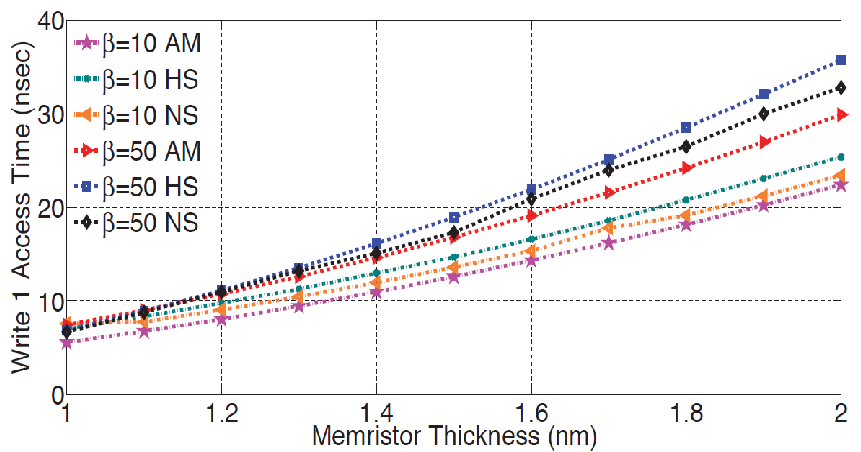
\includegraphics[scale=.35]{writeTime.png}
  \caption{Analytical model vs HSPICE simulations for write 1
access time as a function of memristor thickness for different
$\beta$. AM = Analytical model ignoring bitline capacitance,
HS = Hspice simulations and NS = Numerical solution
accounting for bitline capacitance.}
  \label{fig:writeTime}
\end{figure}
The equation to model the time necessary to write is:
\begin{equation*}
T_{w} = \frac{L^2 (1 + \beta}{2 \mu _{v} V_{A}}
\end{equation*}
$L$ is the thickness of the memristor, $\beta$ is the ratio of $R_{Off}$ and $R_{On}$, $V_{A}$ is the magnitude of the applied voltage, and $\mu _{v}$ is a constant for the mobility of the oxygen vacancy.  According to this equation then, if the thickness of the memristor or the difference in resistance between an off state and on state increase, then the time to write will increase.  If the applied voltage is increased the time to write will decrease.  Using this model a read time of approx. 7 ns was found with $\beta = 10$ and $L = 1 nm$ when writing a 1, but when writing a 0 with the same parameters it can be as low as 4 ns.

\subsubsection{Read Time Model}

\begin{figure}
  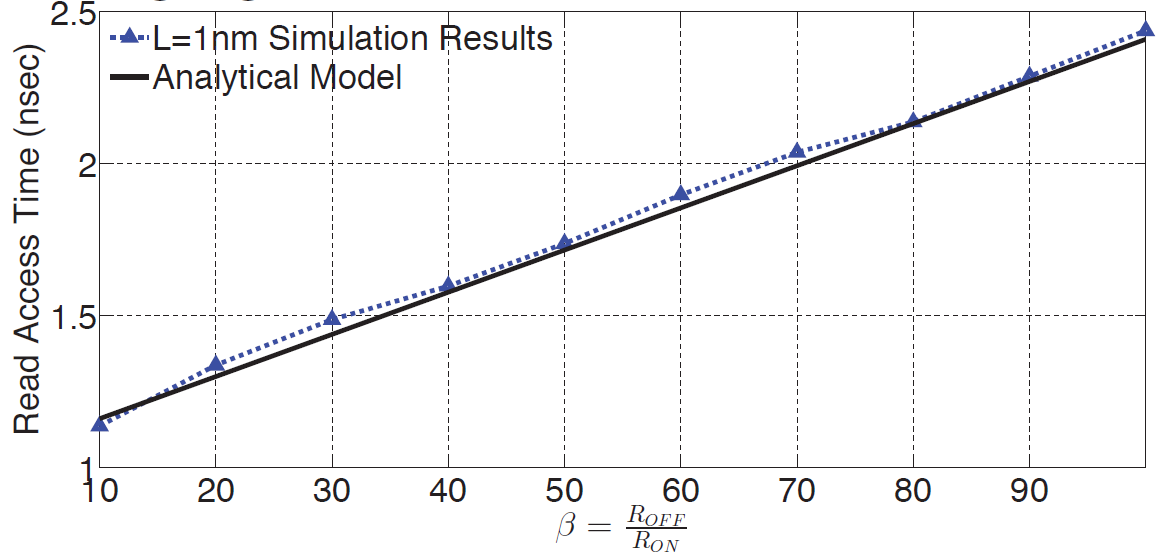
\includegraphics[scale=.29]{readTime.png}
  \caption{Read time model: Analytical model versus HSPICE simulation results
for read access time of the 1T1R cell as a function of $\beta$ for
different memristor thicknesses L.}
  \label{fig:readTime}
\end{figure}
The equation to model the time required to read is:
\begin{equation*}
T_{R} = 0.69(R_{ch} + R_{BL} + R_{Off})C_{BL}
\end{equation*}
$R_{ch}$ is the resistance of the access transistor, $R_{BL}$ is the resistance of the bitline resistor, and $C_{BL}$ is the bitline capacitance. Figure \ref{fig:readTime} provides an illustration with $R_{ON}$ = 100 ohms, $R_{tg}$ = 582 ohms , and  $C_{BL}$ = 200 fF.

\subsubsection{Write Energy Model} 
\begin{figure}
  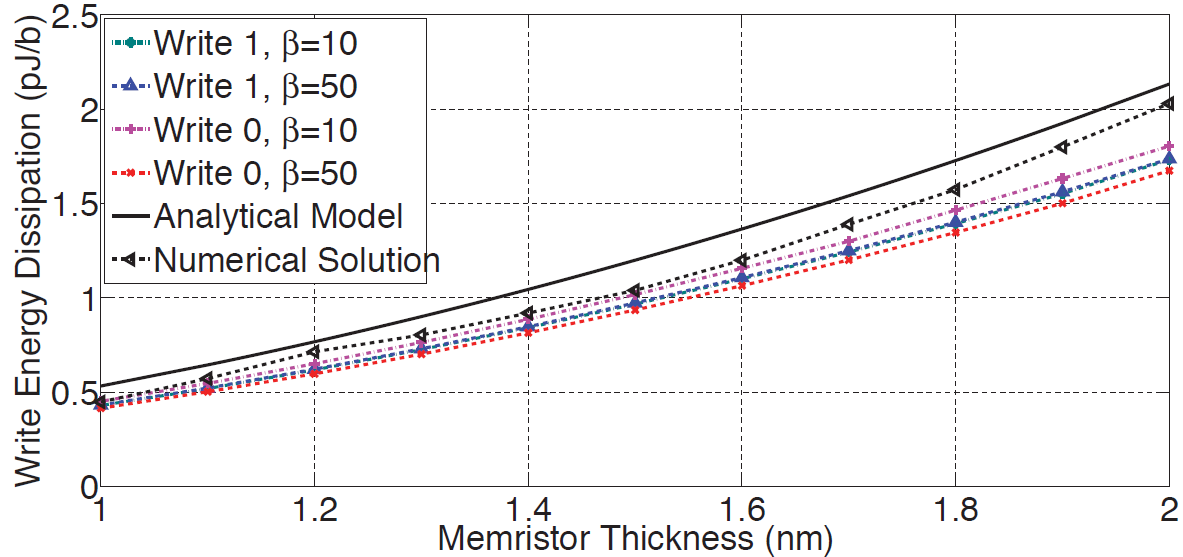
\includegraphics[scale=.29]{writeEnergy.png}
  \caption{ Write Energy Model: AM = Analytical model ignoring the bitline capacitance and NS = Numerical solution considering bitline capacitance.}
  \label{fig:writeEnergy}
\end{figure}
The model for energy consumption during a write procedure is:
\begin{equation*}
E_{w} = \frac{V_{DD}I_{1}}{2(\zeta)}
\end{equation*}
$I_{1}$ is $\int_{.1}^{.9} \frac{1}{1-x^4} dx$, the integral of the inverse of the window function which models the nonlinear rate of state change of a memristor and $\zeta = \frac{\mu _{v}R_{ON}}{L^2}$.  Figure \ref{writeEnergy} graphs the model as a function of memristor thickness with $(Rtg = 582 ohms$, $RON = 100 ohms ,$ and $CBL = 200fF)$.

\subsubsection{Read Energy Model} 
\begin{figure}
  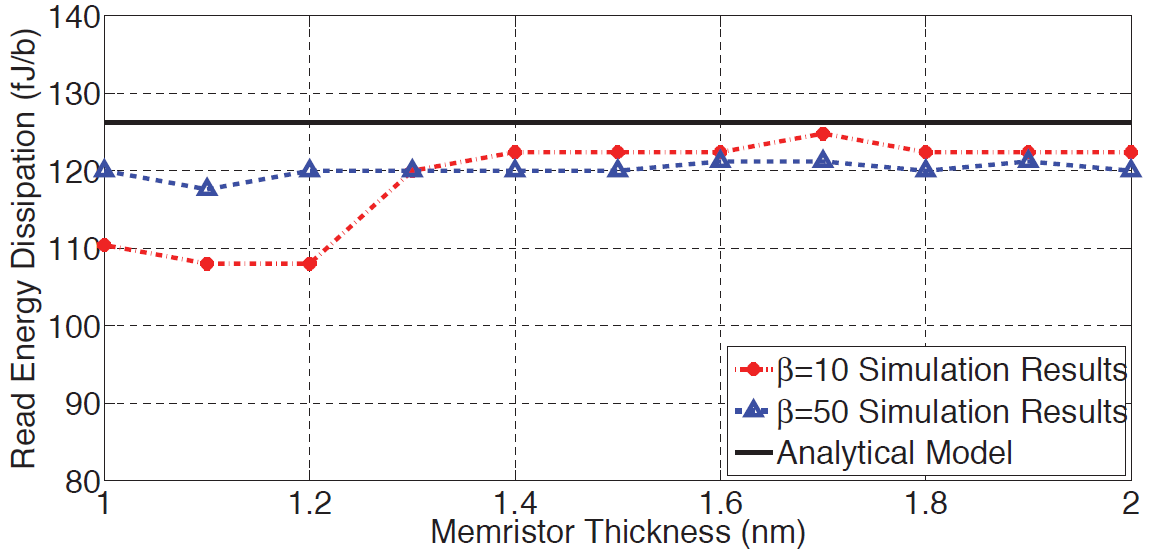
\includegraphics[scale=.29]{readEnergy.png}
  \caption{Energy Model: }
  \label{fig:readEnergy}
\end{figure}
The model for energy consumption during a read procedure is:
\begin{equation*}
E_{R} = 0.63C_{BL}V^2_{DD}
\end{equation*}
Figure \ref{fig:readEnergy} provides a graph of the model, with $R_{On} = 100 ohms $, $C_{BL} = 200fF$, which shows that the energy to read is independent of memristor thickness.
\section{Conclusions}
\label{sec:conclusions}


\section*{Acknowledgments}
\label{sec:acknowledgments}



% The following two commands are all you need in the
% initial runs of your .tex file to
% produce the bibliography for the citations in your paper.
\bibliographystyle{abbrv}
% sample_paper.bib is the name of the BibTex file containing the
% bibliography entries. Note that you *don't* include the .bib ending here.
\bibliography{sample_paper}  
% You must have a proper ".bib" file
%  and remember to run:
% latex bibtex latex latex
% to resolve all references

\end{document}
